\documentclass[12pt]{article}
\usepackage{float}
\usepackage{harvard}
\usepackage[acronym]{glossaries}
\usepackage[automake]{glossaries-extra}
\usepackage[table,xcdraw]{xcolor}
\usepackage{pgfgantt}
\usepackage{graphicx}
\usepackage{array}
\usepackage{multirow}
\usepackage{pdflscape}
\usepackage{pdfpages}
\usepackage[hidelinks]{hyperref}
\usepackage{listings}
\usepackage{xcolor}
\usepackage[noabbrev,capitalize,nameinlink]{cleveref}

\graphicspath{ {./images/} }


\makeglossaries

\newglossaryentry{ictal}
{
        name=latex,
        description={Is a mark up language specially suited for 
scientific documents}
}

\newglossaryentry{preictal}
{
        name=latex,
        description={Is a mark up language specially suited for 
scientific documents}
}

\definecolor{codegreen}{rgb}{0,0.6,0}
\definecolor{codegray}{rgb}{0.5,0.5,0.5}
\definecolor{codepurple}{rgb}{0.58,0,0.82}
\lstdefinestyle{pythonstyle}{
  language=Python,
  basicstyle=\small\ttfamily,
  commentstyle=\color{codegreen},
  keywordstyle=\color{blue},
  numberstyle=\tiny\color{codegray},
  stringstyle=\color{codepurple},
  breaklines=true,
  breakatwhitespace=true,
  numbers=left,
  numbersep=5pt,
  showstringspaces=false,
  tabsize=4,
}

\lstdefinestyle{logstyle}{
  basicstyle=\small\ttfamily,
  breaklines=true,
  breakatwhitespace=true,
  numbers=none, % No line numbers for log output
  frame=none, % No frame for log output
}

%\acrshort{gcd}
%\acrfull{gcd}
\newacronym{eeg}{EEG}{Electroencephalogram}
\newacronym{eegs}{EEGs}{Electroencephalograms}
\newacronym{ai}{AI}{Artificial Intelligence}
\newacronym{ml}{ML}{Machine Learning}
\newacronym{snr}{SNR}{Signal-to-Noise Ratio}
\newacronym{emd}{EMD}{Empirical Mode Decomposition}
\newacronym{imf}{IMF}{Intrinsic Mode Functions}
\newacronym{csp}{CSP}{Common Spatial Pattern}
\newacronym{ga}{GA}{Genetic Algorithm}
\newacronym{loocv}{LOOCV}{Leaving One Out Cross-Validation}
\newacronym{ann}{ANN}{Artificial Neural Network}
\newacronym{mlpann}{MP-ANN}{Multi-layer Perceptron Artificial Neural Network}
\newacronym{dwt}{DWT}{Discrete Wavelet Transformation}
\newacronym{rnn}{RNN}{Recurrent Neural Network (Elman)}
\newacronym{cnn}{CNN}{Convolutional Neural Network}
\newacronym{svm}{SVM}{Support Vector Machine}
\newacronym{knn}{kNN}{K Nearest Neighbor}
\newacronym{lr}{LR}{Logistical Regression}
\newacronym{pca}{PCA}{Principal Component Analysis}
\newacronym{rf}{RF}{Random Forest}
\newacronym{memd}{MEMD}{Multivariate Empirical Mode Decomposition}
\newacronym{stft}{STFT}{Short-Time Fourier Transform}
\newacronym{chb}{CHB-MIT}{Children's Hospital Boston}
\newacronym{edf}{EDF}{European Data Format}

\title{Real-time preictal detection through the application of machine learning to Electroencephalogram signals.}
\author{William Riddell}
\date{\parbox{\linewidth}{\centering
\vspace{0.5cm}
\today\endgraf\bigskip\vspace{0.5cm} 
Word Count: 10,000 \\ \vspace{0.5cm}  
Supervised by Kashinath Basu}}



\begin{document}
%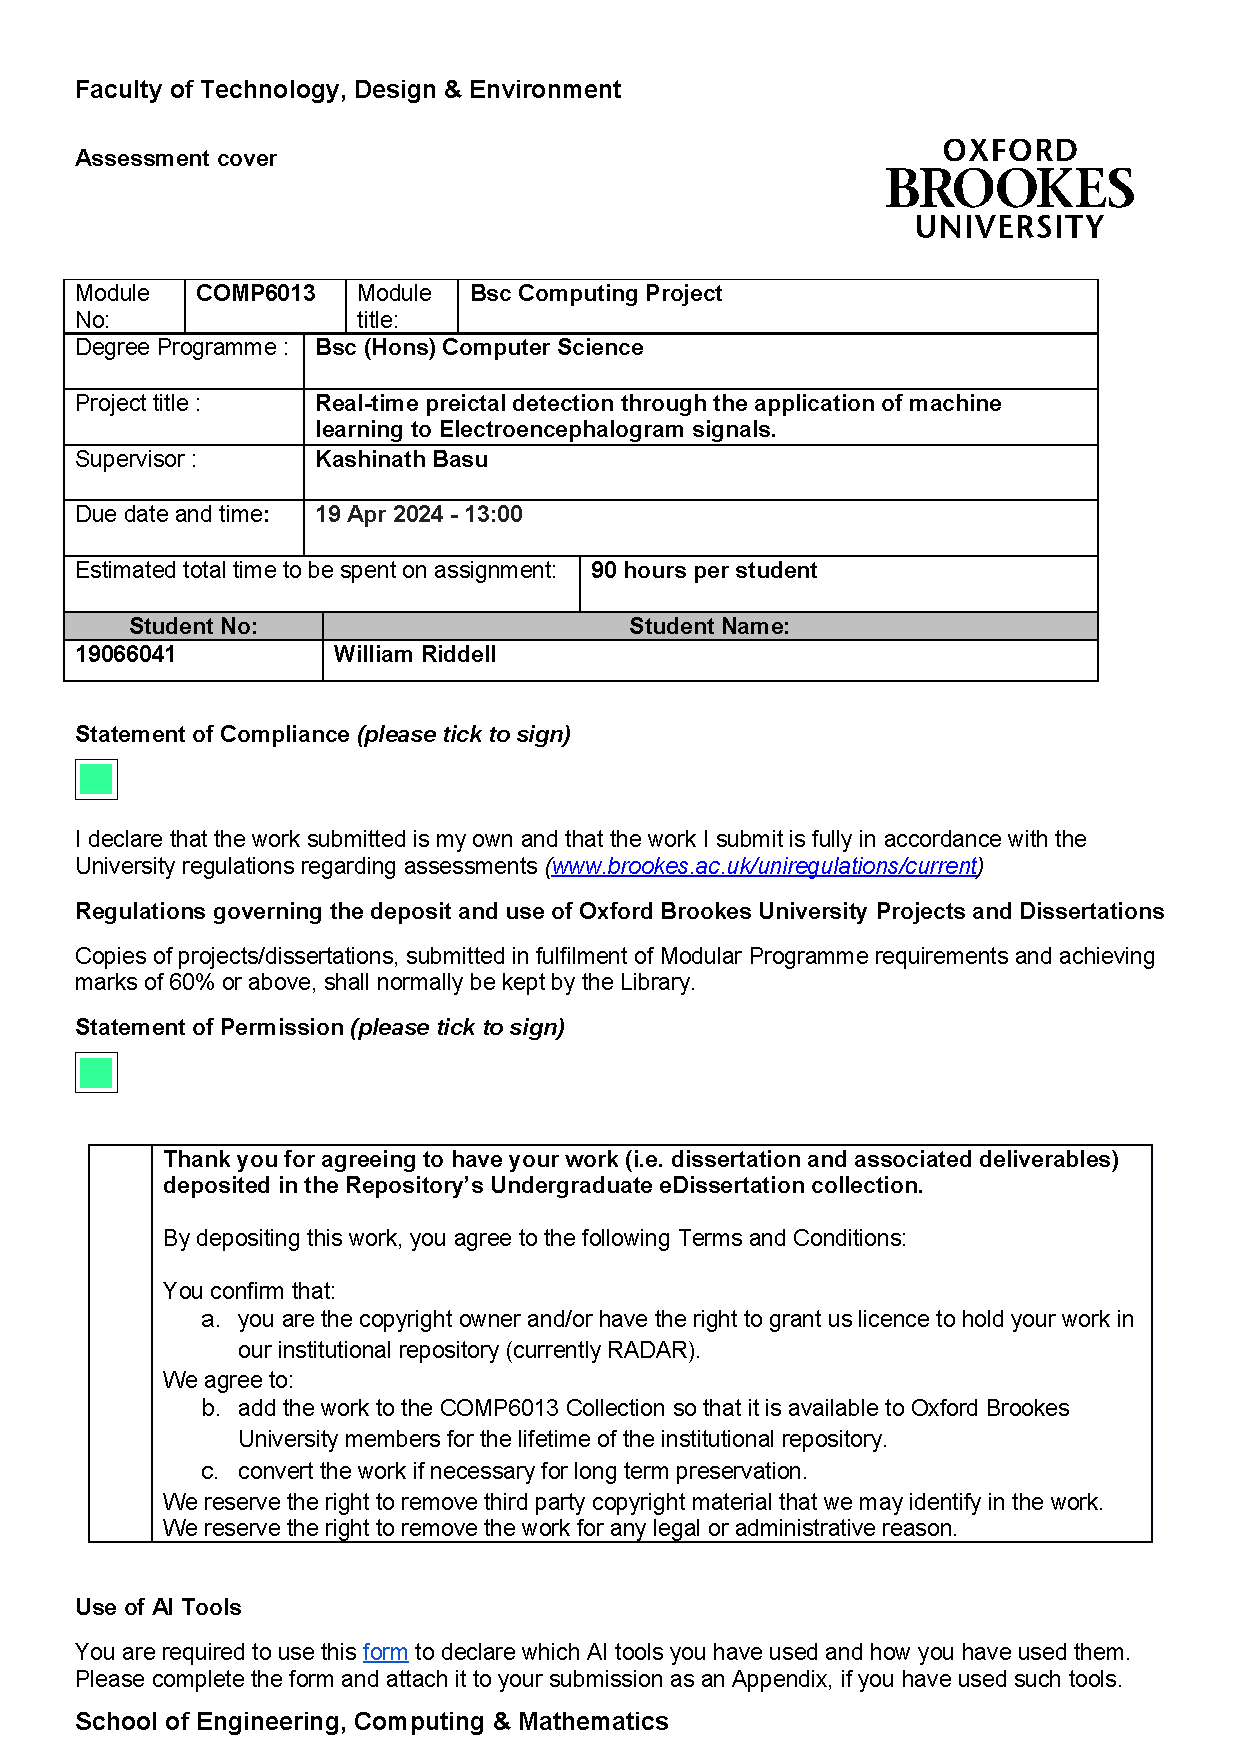
\includepdf[pages=-]{cover.pdf}
\maketitle

\vfill 
\begin{center} 
Faculty of Technology, Design and Environment\\
School of Engineering, Computing and Mathematics
\end{center}
\pagebreak
\tableofcontents
\printglossary[type=\acronymtype]
\pagebreak


\section{Abstract}

asdf









\section{Acknowledgements}

asdf








\section{Introduction}


Over the last 20 years, \acrfull{ai} has seen a large evolution through the use of \acrfull{ml}; the statistical analysis of data which leads to the unveiling of characteristics and connections. \cite{awad2015efficient}. There has been a large uptake of applying \acrshort{ml} techniques to biomedical data, increasing the speed and accuracy of prediction, detection, diagnosis, and prognosis. 

\acrfull{eegs} measure the electrical signals in the brain. \acrshort{eegs} have a great use in giving an insight into the inner workings of the brain, for example allowing us to pick up abnormalities preceding and during their occurrence. ``A seizure is a burst of uncontrolled electrical activity between brain cells (also called neurons or nerve cells) that causes temporary abnormalities in muscle tone or movements (stiffness, twitching or limpness), behaviours, sensations or states of awareness.'' \cite{johnHopkinsTypesOfSeizures} Due to this, monitoring the brain's electrical activity through the use of an \acrshort{eeg}, and applying analysis through an \acrshort{ml} model may allow us to detect the preictal period. ``An automated accurate prediction of seizures will significantly improve the quality of life of patients and reduce the burden on caregivers'' \cite{acharya2018automated}


\subsection{Background}

``Because of their unpredictable nature, uncontrolled seizures represent a major personal handicap and source of worry for patients. In addition, persistent seizures constitute a considerable burden on healthcare resources.'' \cite{assi2017towards} Due to this both medication and surgery are available to applicable patients, although with ~30\% patients being refractory to drug therapy, and an equally bleak surgery success rate; ~75\% in lesional cases, and ~50\% in nonlesional cases for temporal lobe cases along with ~60\% in lesional cases and merely ~35\% in nonlesional for frontal lobse cases \cite{assi2017towards}, a large population of patients would therefore greatly benefit from a prediction system in their daily life. 

\subsection{Aim and Objectives}

This project will aim to develop an consistent \acrshort{ml} model trained to classify either preictal, interictal and ictal periods. The model will have to achieve a high degree of accuracy ($\geq90\%$) when being applied to \acrshort{eeg} data in real-time. Furthermore a real-time simulation will need to be developed along with an \acrshort{ml} pipeline and model parameter tuning. 

 
\paragraph{Objectives}

\begin{enumerate}
        \item Create a preprocessing pipeline which extracts the dataset into an \acrshort{ml} format suitable for training. The process should be efficient enough to meet the real-time requirements. 
        \item Review previous papers to compare previous \acrshort{ml} model approaches and compare their performance.
        \item Tune the hyper-parameters of the selected \acrshort{ml} model approach.
        \item Produce a simulation interface which streams \acrshort{eeg} data in real time through the preprocessing pipeline and into an model, showing the current classification to the user.
\end{enumerate}

\subsection{Project Requirements}


The final product needs to have the ability to accept a stream of raw EEG data, it will need to run the data through a preprocessing pipeline and then through a model. It will need to display the current classification to the user. This process should update at least once a second. The final model is also required to have a classification accuracy of $\geq90\%$. 


\section{Background Review}

\subsection{Datasets}

\cite{wong2023eeg} reviews 10 datasets available to download. It evaluates the way the \acrshort{eegs} were physically setup on the subject, the subjects themselves and the data's properties. Wong et al. also states their opinion on what tasks suit what dataset, with the main two tasks being either detection or prediction. 

\begin{table}[H]
\centering
\begin{tabular}{l}
\textbf{Dataset}                       \\
University of Bonn                   \\
CHB-MIT Scalp EEG                    \\
Melbourne-NeuroVista seizure trial (Neurovista Ictal)                           \\
Kaggle UPenn and Mayo Clinic's Seizure Detection Challenge                     \\
Neurology and Sleep Centre Hauz Khas \\
Kaggle American Epilepsy Society Seizure Prediction Challenge                  \\
Kaggle Melbourne-University AES-MathWorks-NIH Seizure Prediction Challenge \\
TUH EEG Seizure Corpus (TUSZ)        \\
Siena Scalp EEG                      \\
Helsinki University Hospital EEG    
\end{tabular}
\caption{The Datasets analysed}
\end{table}

Within these datasets Wong et al. was also able to find the way the EEG nodes were positioned on the subject's cranium, along with whether the EEG nodes were either placed intracranial or extracranial. Wong et al. also the number of channels that are contained in the raw EEG data for each dataset.

\begin{table}[H]
\centering
\begin{tabular}{p{0.4\textwidth}p{0.1\textwidth}p{0.2\textwidth}p{0.2\textwidth}}
\textbf{Dataset}                                              & \textbf{Number of channels} & \textbf{Placement method}                & \textbf{Type of signal} \\
University of Bonn                                            & 1                           & International 10–20 system, Intracranial & Scalp/Intracranial EEG  \\
CHB-MIT Scalp EEG                                             & 18                          & International 10–20 system/Nomenclature  & Scalp EEG               \\
Melbourne-NeuroVista seizure trial (NeuroVista Ictal)         & 16                          & Intracranial                             & Intracranial EEG        \\
Kaggle UPenn and Mayo Clinic's Seizure Detection Challenge    & 16–76                       & Intracranial                             & Intracranial EEG        \\
Kaggle American Epilepsy Society Seizure Prediction Challenge & 16                          & Intracranial                             & Intracranial EEG        \\
Neurology and Sleep Centre Hauz Khas                          & 1                           & International 10–20 System               & Scalp EEG               \\
Kaggle Melbourne-University AES-MathWorks-NIH Seizure Prediction Challenge Data & 16 & Intracranial & Intracranial EEG \\
TUH EEG Seizure Corpus (TUSZ)                                 & 23–31                       & International 10–20 system / Nomenclature & Scalp EEG               \\
Helsinki University Hospital EEG                              & 19                          & International 10–20 system               & Scalp EEG               \\
Siena Scalp EEG                                               & 20/29                       & International 10–20 system/Nomenclature  & Scalp EEG              
\end{tabular}
\caption{Channel Characteristics}
\end{table}

Wong et al. also noted along with this data that the ``University of Bonn dataset contains a mixture of both scalp and intracranial EEG data where scalp EEG from healthy subjects was taken, while intracranial EEG was taken from subjects with a history of seizures.'' \cite{wong2023eeg}. This may present a skew on the \acrshort{ml} model during training.


\begin{table}[H]
\centering
\begin{tabular}{p{0.4\textwidth}p{0.2\textwidth}p{0.2\textwidth}p{0.2\textwidth}}
  \textbf{Dataset} &
  \textbf{Noncontinuous data} &
  \textbf{Short-term continuous data} &
  \textbf{Continuous data} \\
  
University of Bonn                                                              & Yes & No  & No  \\
CHB-MIT Scalp EEG                                                               & No  & Yes & Yes \\
Melbourne-NeuroVista seizure trial (Neurovista Ictal)                           & N/A & N/A & N/A \\
Kaggle UPenn and Mayo Clinic's Seizure Detection Challenge                      & Yes & No  & No  \\
Kaggle American Epilepsy Society Seizure Prediction Challenge                   & Yes & No  & No  \\
Neurology and Sleep Centre Hauz Khas                                            & Yes & No  & No  \\
Kaggle Melbourne-University AES-MathWorks-NIH Seizure Prediction Challenge Data & Yes & No  & No  \\
TUH EEG Seizure Corpus (TUSZ)                                                   & No  & Yes & No  \\
Helsinki University Hospital EEG                                                & No  & Yes & No  \\
Siena Scalp EEG                                                                 & No  & Yes & No 
\end{tabular}
\caption{Temporal properties}
\end{table}

Wong et al. ordered the datasets into groups, either continuous or non continuous data. For the continuous data they separated out datasets which record for less that 24 hours in a single go, these were classified as ``Short-term continuous'' data.

\begin{table}[H]
\centering
\begin{tabular}{p{0.4\textwidth}p{0.2\textwidth}p{0.2\textwidth}p{0.2\textwidth}}
\textbf{Dataset}                                                                & \textbf{Number of subjects} & \textbf{Subject type} & \textbf{} \\
University of Bonn                   & 10  & Human &  \\
CHB-MIT Scalp EEG                    & 23  & Human &  \\
Melbourne-NeuroVista seizure trial (NeuroVista Ictal)                           & 12                          & Human                 &           \\
Kaggle UPenn and Mayo Clinic's Seizure Detection Challenge                      & 12                          & Human \& Canine       &           \\
Kaggle American Epilepsy Society Seizure Prediction Challenge                   & 7                           & Human \& Canine       &           \\
Neurology and Sleep Centre Hauz Khas & 10  & Human &  \\
Kaggle Melbourne-University AES-MathWorks-NIH Seizure Prediction Challenge Data & 3                           & Human                 &           \\
TUH EEG Seizure Corpus (TUSZ)        & 642 & Human &  \\
Helsinki University Hospital EEG     & 79  & Human &  \\
Siena Scalp EEG                      & 14  & Human & 
\end{tabular}
\caption{Subject properties}
\end{table}

Wong et al. also was able to identify the number of subjects within each dataset. Within the two ``Kaggle'' datasets there are Canine subjects, making them unsuitable for this project. 

Within the review, they also produced tables displaying the segment information for each dataset, breaking down the recording length and frequency, along with the number of events and segments. This information should not weight into which dataset suits the idea of preictal prediction so shall be left out in this background review. Wong et al. also discussed the idea of the class imbalance problem, where the number and length of each ictal period is unbalanced. Two datasets, ``University of Bonn'' and the ``Neurology and Sleep Centre Hauz Khas'' have addressed this issue and have balanced their data between ictal, preictal, interictal and nonictal periods.

Taking the research into account Wong et al. suggested which dataset suits either prediction or detection. ``Since the aim of seizure prediction is to forecast impending seizures, EEG recordings that include preictal and interictal data should be used for the study, while the aim of seizure detection is to detect ongoing seizure events, hence, EEG recordings that contain ictal and interictal data should be used.'' \cite{wong2023eeg}.

\begin{table}[H]
\centering
\begin{tabular}{p{0.5\textwidth}p{0.4\textwidth}}
\textbf{Dataset}                     & \textbf{Application}         \\
University of Bonn                   & Seizure detection            \\
CHB-MIT Scalp EEG                    & Seizure detection/Prediction \\
Melbourne-NeuroVista seizure trial (NeuroVista Ictal)                           & Seizure detection/Prediction \\
Kaggle UPenn and Mayo Clinic's Seizure Detection Challenge                      & Seizure detection            \\
Kaggle American Epilepsy Society Seizure Prediction Challenge                   & Seizure prediction           \\
Neurology and Sleep Centre Hauz Khas & Seizure detection/Prediction \\
Kaggle Melbourne-University AES-MathWorks-NIH Seizure Prediction Challenge Data & Seizure prediction           \\
TUH EEG Seizure Corpus (TUSZ)        & Seizure detection/Prediction \\
Helsinki University Hospital EEG     & Seizure detection/Prediction \\
Siena Scalp EEG                      & Seizure detection/Predictio 
\end{tabular}
\caption{Suggested applications}
\end{table} 

\subsection{\acrfull{ml} Models}

A series of papers have been reviewed with the following \acrshort{ml} model types being used:

\begin{itemize}
	\item \acrfull{knn}
	\item \acrfull{svm}
	\item \acrfull{lr}
	\item \acrfull{rf}
	\item \acrfull{ann}
	\item \acrfull{cnn}
\end{itemize}

\paragraph{\acrfull{knn}}\mbox{}\\


\cite{wang2013online} shows an \acrshort{knn} classifier being used which lead to a sensitivity of 73\% and a specificity of 67\% when using the estimation of short term maximum lyapunov exponent.


\paragraph{\acrfull{svm}}\mbox{}\\


Various \acrshort{svm} classifiers were found to be used, one of which was by \cite{cho2016eeg} which used both clinical and generated data, where the training data was filtered using BPF, EMD, MEMD and NA-MEMD. Features were then extracted through \acrshort{emd}, \acrshort{memd}, and frequency selection.\cite{cho2016eeg} was able to achieve a classification rate of around 80\%.

\paragraph{\acrfull{lr}}\mbox{}\\

Mirowski et al. used a combination of \acrshort{lr} and \acrshort{svm} classifiers to achieve a 71\% accuracy along with 0 false positives \cite{mirowski2009classification}.

\paragraph{\acrfull{rf}}\mbox{}\\

Jacobs et al. used a \acrshort{rf} derived approach which was a multistage classification system that used cross-frequency coupling. Jacobs et al. was able to achieve an impressive 87.9\% sensitivity, and an 93.4\% area-under-the-ROC \cite{jacobs2018classification}.

\paragraph{\acrfull{ann}}\mbox{}\\

\acrshort{ann} have enabled researchers to develop increasingly accurate models. \cite{sharma2018epileptic} shows this in their results boasting an accuracy of 92.3\% and an sensitivity of 100\%. Sharma however did use 72 parameters for classification. 

\paragraph{\acrfull{cnn}}\mbox{}\\

Various \acrshort{cnn} have been developed, with most of them showing promising results. An example of this was from \cite{mirowski2009classification}, using the same dataset Mirowski et al. used to train their \acrshort{rf} based model off, they were able to achieve a 100\% prediction rate for 15 out of their 21 patients, along with 0 false positives. 

It should be noted, that Mirowski et al. training this model for a per patient basic, and suggested that each patient has their own compilation of models trained to them for the highest chance of prediction, along with minimal false positives. 





\section{Project Methodology and Development}

\subsection{Decisions}

\subsubsection{Approach}

Through the analysis of various \acrshort{ml} models an \acrshort{cnn} will be used for this project. Mirowski et al. were able to achieve an accuracy that meets the project's requirements making it a valid choice. <paper> also used an \acrshort{cnn}, but with an image classification. This approach was able to achieve similar results while being less computationally intense. This combination was therefore chosen as the base for this project. 

From the datasets discussed the \acrfull{chb} \acrshort{eeg} dataset has been chosen due to the large amount of continuous data, suitable for extracting the preictal period. The dataset also has \acrshort{eeg} nodes positioned on the subject's scalps, fitting with the use case of this project. Furthermore, the \acrshort{chb} \acrshort{eeg} dataset has produced summary plain-text files for each of the subject's recordings, stating when every seizure began and ended. 

\subsubsection{Development System}

Due to the linear nature of this project an Waterfall methodology will be used. Waterfall ensures that previous stages of the software are complete before moving on, this will keep the project on track and moving in an forward direction, crucial for the time-limited aspect of this project. Furthermore, due to the analysis undergone through literature reviews the direction and therefore the goals of the project are clearly defined; this further supports the choice of an Waterfall approach.  

\subsubsection{Version Control}

This project will be under version control through the use of Git, along with GitHub as an remote repository. Both the dataset and the trained models will not be under version control. The use of an version control system and remote repository ensures that if anything goes awry an backup of all commits are stored remotely, securing any progress made in the project. Git also gives the benefit of many features; notably branches and stashing, allowing for developing on ideas, features, and bugs without affecting the ``main'' code, and merging allows for the combination of said branches. 

\subsubsection{Software and Libraries Used}

\begin{table}[H]
\centering
\begin{tabular}{p{0.3\textwidth}p{0.7\textwidth}}
Name:              & Use case:                                                                                                                               \\
Google Cloud       & Used to download the \acrshort{chb} \acrshort{eeg} dataset                                                                            \\
Keras (TensorFlow) & Used to build, train and test the \acrshort{ml} models.                                                                \\
Matplotlib         & Used in the real-time simulation to plot the Spectrogram and \acrshort{chb} \acrshort{eeg} data.                                       \\
MNE                & Provides classes for loading \acrshort{eeg} data from both CSV and \acrshort{edf} files. Also used for running an \textbackslash{}acrfull\{stft\} extraction. \\
NumPy              & Utilized functions and classes to store and manipulate loaded data.                                                                     \\
Pandas             & Utilized functions and classes to store and manipulate loaded data.                                                                     \\
scikit-learn       & Provides functions used to produce performance metrics for trained \acrshort{ml} models.                              
\end{tabular}
\caption{List of Libraries used}
\label{tab:libraries}
\end{table}


\subsubsection{Schedule}

The schedule describes the way the Waterfall methodology has affected the project; it shows how it's been broken down into smaller, distinct stages with progress being blocked until the previous stage has been completed. The overlap in March and April is when the models are being tuned, therefore the only active development is on the real-time simulation. 

\begin{figure}[H]
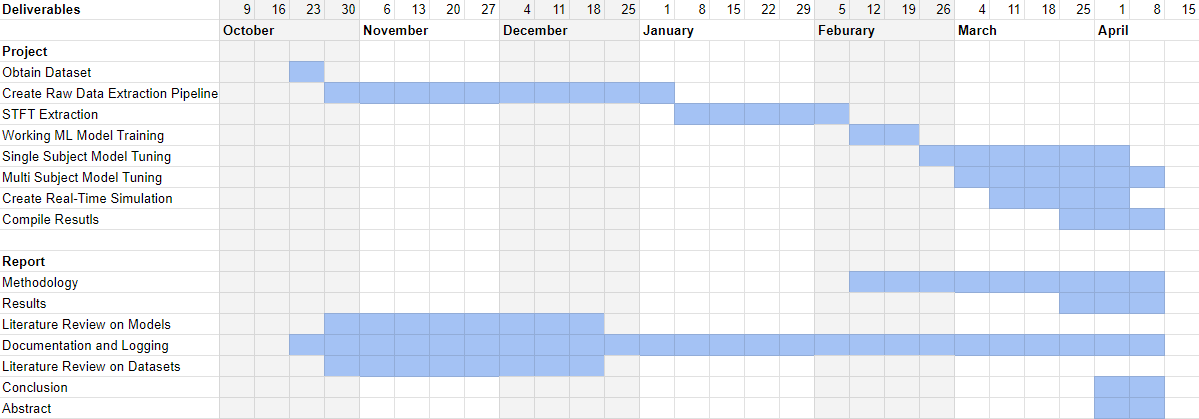
\includegraphics[width=\textwidth]{gantt}
\centering
\caption{Gantt Chart}
\label{fig:gantt}
\end{figure}


\subsection{Development}

\subsubsection{Raw Data Extraction}

The \acrfull{edf} \cite{kemp1992simple} is a computer file format that was originally designed for archival and exchange  of ... recordings. \cite{kemp2013european}. This was the chosen format from the \acrshort{chb} \acrshort{eeg} dataset along with corresponding summary files see \ref{lst:summary-file}. From these summary files and the data stored in the \acrshort{edf} files an OOP representation of the dataset was created, containing the channels (individual \acrshort{eeg} nodes), recording frequency, and seizure start and end times. With this OOP representation the raw data was extracted from the \acrshort{edf} files. Using the OOP representation the ictal, preictal and interictal periods for each recording were extracted and saved in corresponding directories. Furthermore, only the common channels between all subjects were extracted, following the international 10-20 layout, these were the 17 channel names: FP1-F7, F7-T7,T7-P7, P7-O1, FP1-F3, F3-C3, C3-P3, P3-O1, FP2-F4, F4-C4, C4-P4, P4-O2, FP2-F8, F8-T8, P8-O2, FZ-CZ, CZ-PZ.

\subsubsection{\acrfull{stft}}

For each subject \acrshort{stft} is applied to the data collected from the \acrshort{eegs} to produce an spectrogram of length 30 seconds. These images contains only a single class and were the input into the \acrshort{cnn}. \acrshort{stft} can be expressed mathematically;\\ 

$$ \mathbf{STFT}\{x(t)\}(\tau,\omega) \equiv X(\tau, \omega) = \int_{-\infty}^{\infty} x(t) w(t-\tau) e^{-i \omega t} \, d t  $$


Where $w(\tau)$ is an window function and $x(t)$ is the input signal from the \acrshort{eegs}.\\


This can also be explained as taking an Fourier transform of the \acrshort{eeg} signals after an window function has been applied, and then sliding an window across the result. The sliding window transforms the one-dimensional output from the Fourier transform into two-dimensional data allowing for visual analysis. 


There are various parameters for an \acrshort{stft} transformation: 
\begin{table}[H]
\centering
\begin{tabular}{p{0.3\textwidth}p{0.7\textwidth}}
Window Function & Used to isolate signal currently undergoing analysis. Optimal functions have low to no artefacts left in the signal and creates no discontinuities at section boundaries.\\
Window Size & Changes the size of the window function. This affects the resolution of both time and frequency, leading to the uncertainty principal; either variable will be in high resolution. See \ref{fig:stft1} and \ref{fig:stft2} \\
Time Step (step size or hop size) & This is the distance between windows. Influences window over or underlap, as well as directly affecting computational load. \\                            
\end{tabular}
\caption{List of \acrfull{stft} parameters}
\label{tab:stft_params}
\end{table}

For this project these variables were selected:

\begin{table}[H]
\centering
\begin{tabular}{p{0.3\textwidth}p{0.7\textwidth}}
Window Function & Sine Window: $ w[n] = \sin\left(\frac{\pi n}{N}\right) = \cos\left(\frac{\pi n}{N} - \frac{\pi}{2}\right),\quad 0\le n \le N.$ \\
Window Size & 7680. The length of the input data. \\
Time Step (step size or hop size) & 3840. This leads to an window overlap. \\                            
\end{tabular}
\caption{List of \acrfull{stft} parameters choices}
\label{tab:stft_choices}
\end{table}

See \ref{fig:stft2} for an Spectrogram produced with these parameters. 

\subsubsection{Notch Filter}

``Power line interference may severely corrupt neural recordings at 50/60 Hz and harmonic frequencies. The interference is usually non-stationary and can vary in frequency, amplitude and phase.'' \cite{keshtkaran2014fast} This poses a large issue when training an \acrshort{ml} model against \acrshort{eeg} recordings as the interference may affect the model's ability to pick up on characteristics, or may mislead the model. \ref{fig:stft1} clearly shows power line interference with two horizontal bands around 60 Hz and again around 78 Hz. Due to this power line interference needs to be removed, although the time-sensitive nature of this project meant an resource light method was required. Through analysis done by MR Keshtkaran, Z Yang an notch filter has various drawbacks such as not entirely removing the interference \cite{keshtkaran2014fast}, however for this project the alternatives were too computationally intense to run in an real-time setting. Therefore an notch filter was applied to the raw data before each \acrshort{stft} was applied. 


\subsubsection{Synthesize Data}

There was also a need to synthesize data in order to fix the class imbalance. For some subjects their ictal periods were very short, only a couple of seconds long in some cases, or the ictal periods were $>20$ minutes into the recording leading to the preictal period being cut short. Decreasing the number of \acrshort{stft} spectrograms for each class was not a solution as for most subjects their ictal spectrogram count was insufficient, therefore synthesizing spectrogram windows was required to bring the count for each class inline with the interictal class. This was achieved with an sliding window method, see \ref{fig:slidingWindow}. The sliding window offset was calculated for each subject such that each class had the same number of spectrograms as the interictal period.

\subsubsection{\acrfull{cnn}}

asdf




\subsection{Problems Encountered}

When attempting to gain access to the prediction applicable datasets that were discussed in the literature review, some datasets were not public; Contacting the managing bodies of a few of these datasets did not lead to a response, translating to an reduction of available data to train against. This was a factor when deciding to use the ``CHB-MIT Scalp EEG'' Dataset. This dataset however did not come without its issues.

``CHB-MIT Scalp EEG'' came with a descriptive labelling of each EEG data file. The description of each file included the ictal periods start times, the number of ictal periods, the channel names, and the frequency of the recorded data. Some of the descriptions were not accurate of the raw data it was attempting to describe. An example of this was that the descriptor file contained duplicate channel names. This caused issues when extracting the raw data as the Python 3 library ``mne'' requires unique channel names,  this was easily solved through an implimentation of a naming convention in this case. Another issue which arose was the number of raw channels extracted was greater than the expected number of channels described in the description file. This again caused issues with ``mne''. In these cases however the raw extracted channels contained a basic name that could be used, although for other datasets where this may be an issue another naming convention may have to be implemented. 

Feature extraction has not been fully implemented yet, one of the concerns of feature extraction however will be the speed of the extraction in relation to time, particularly, if the extraction of the statistical features can be done within the frequency of the EEG recording. As the ``CHB-MIT Scalp EEG'' dataset has a frequency of 256hz, feature extraction and also the writing of said features all has to occur within 3.9ms. Due to this a solution will have to be realized. The current approach is to develop a Python3 program to achieve this and benchmark the speed, the expectation is that the Python3 program will be drastically too slow, but gives an indication to if feature extraction can be achieved for each frequency through possibly a C program. If not, other avenues will have to be explored, such as creating hash maps for faster approximated feature extraction, or even sampling a smaller number of recorded rows. \acrfull{pca} may have to be explored here, as extracting fewer features, but for a greater number of frequencies may lead to higher accuracy results, although tuning of features will have to take place after the \acrshort{ml} model experiment.



\subsection{Supervision}

The project supervisor has aided the direction of the project, introducing the idea of setting up the \acrshort{ml} model experiment to evaluate the accuracy of each model. This has lead to further realizations such as \acrshort{pca} experiments which will help solve upcoming issues discussed in the ``Problems Encountered'' section. The project supervisor also gave literature review feedback which pushed me to analyse currently developed systems I would not of otherwise. Weekly meetings with the supervisor kept them informed on the progress of the project, allowing them to give guidance as discussed.


\section{Professional Issues and Risks}

\subsection{Professional Issues}

\begin{enumerate}
    \item Legal Issues:
    \begin{itemize}
        \item There are a few legal issue which are attached to the project. Firstly GDPR rules need to be followed as the data moving into the model for both live classification and training need to be dealt in a legal manner. Data will be stored after classification as this allows for further development of the model, therefore an appropriate timespan will need to be decided before the data needs to be deleted. Along with this, security measures should be implemented to to stop attackers or un-authorized persons viewing or copying the data. The other legal issue which may come into play would be who is liable if a seizure is avoided. This could be solved through an agreement the end user has to accept stating the producers of the product, including the developers as not liable if this occurs as the product will never be truly \%100 accurate.
    \end{itemize}
    \item Social Issues:
    \begin{itemize}
    	 \item People from all walks of life have epilepsy, and due to financial costs some may not be able to afford the final solution. This will be an issue that may not be solvable by the producers of the software, and instead may need to rely on outsourced funding such as the healthcare service. The producers can make the software available, although it will still take time, money, and knowledge for the individual to setup a system that meets the expectations of a finished product. 
    \end{itemize}
        \item Ethical Issues:
    \begin{itemize}
    	 \item The final product should attempt to achieve the same accuracy regardless of age or gender, although due to the differences in the the human brain this may be a difficult task to achieve for a single solution. In an ideal world a model will be trained, focused on different populations to pick up on their differencing characteristics of their preictal periods, although due to the lack of datasets this currently is not achievable until more data is recorded once the initial product has been deployed. 
    \end{itemize}
        \item Environmental Issues:
    \begin{itemize}
    	 \item EEG nodes are comparatively inexpensive to their possible benefits, meaning the creation of the device won't have a large overall cost. The \acrshort{ml} model training however will be computationally expensive, translating to large energy usage, therefore ways to minimize energy consumption when training the \acrshort{ml} model should be taken into account for the final product. 
    \end{itemize}
            \item Intellectual Property Issues:
    \begin{itemize}
    	 \item There will be an issue when deciding who owns the recorded data. If the company who produces the final product owns it then they can utilize the large amount of data to further refine and train more advanced models, allowing them to tackle other issues such as the ones discussed in ``Social Issues'', although this should be a choice for the end user. Another issue may be patenting the final product and which components should be patented or copyrighted such if the most recent model or older versions will be freely available, or if they will be closed sourced. 
    \end{itemize}
        \item Accessibility Issues:
    \begin{itemize}
    	 \item As discussed epileptic patients come from all walks of life which means the final device needs to have an accessible interface, allowing everyone to have a clear indication of the state of the device, including the preictal period alert or even if the device is on. Different people will need different alert methods, and the final device should be extensible, allowing the final patient to fit it to their disability. Some variants of the device should have any combination of light, sound and vibration alert, as well as notifications to any of their devices. 
    \end{itemize}
\end{enumerate}

\subsection{Risks}

\subsubsection{Risk Matrix}

The numbers in each cell of the risk matrix corresponds to the items in the risk assessment. 

\begin{table}[H]
\centering
\begin{tabular}{l|llll}
                              & \multicolumn{4}{l}{Harm Severity}                                                                                                                                                             \\
\multirow{-2}{*}{Probability} & \multicolumn{1}{l|}{Minor}                    & \multicolumn{1}{l|}{Marginal}                 & \multicolumn{1}{l|}{Critical}                 & \multicolumn{1}{l|}{Catastrophic}             \\ \hline
Certain                       & \multicolumn{1}{l|}{\cellcolor[HTML]{FE996B}} & \multicolumn{1}{l|}{\cellcolor[HTML]{FE996B}} & \multicolumn{1}{l|}{\cellcolor[HTML]{FD6864}} & \multicolumn{1}{l|}{\cellcolor[HTML]{FD6864}} \\ \hline
Likely                        & \multicolumn{1}{l|}{\cellcolor[HTML]{FFFE65}} & \multicolumn{1}{l|}{\cellcolor[HTML]{FE996B}} & \multicolumn{1}{l|}{\cellcolor[HTML]{FE996B}} & \multicolumn{1}{l|}{\cellcolor[HTML]{FD6864}} \\ \hline
Possible                      & \multicolumn{1}{l|}{\cellcolor[HTML]{67FD9A}} & \multicolumn{1}{l|}{\cellcolor[HTML]{FFFE65}} & \multicolumn{1}{l|}{\cellcolor[HTML]{FE996B}} & \multicolumn{1}{l|}{\cellcolor[HTML]{FD6864}} \\ \hline
Unlikely                      & \multicolumn{1}{l|}{\cellcolor[HTML]{67FD9A}} & \multicolumn{1}{l|}{\cellcolor[HTML]{FFFE65}} & \multicolumn{1}{l|}{4, 6\cellcolor[HTML]{FFFE65}} & \multicolumn{1}{l|}{3, 5, 7\cellcolor[HTML]{FE996B}} \\ \hline
Rare                          & \multicolumn{1}{l|}{\cellcolor[HTML]{67FD9A}} & \multicolumn{1}{l|}{\cellcolor[HTML]{67FD9A}} & \multicolumn{1}{l|}{\cellcolor[HTML]{FFFE65}} & \multicolumn{1}{l|}{1, 2\cellcolor[HTML]{FFFE65}} \\ \hline
\end{tabular}
\caption{Risk Matrix}
\label{tab:risk-matrix}
\end{table}


\subsubsection{Risk Assessment}


The risks proposed are for a final product which is available to consumers who suffer from epilepsy as well as healthcare services. The current scope of the project does not affect the risks stated above, and therefore the development goals have not been changed to negate any of these risks.

\begin{table}[H]
\centering
\begin{tabular}{p{0.03\linewidth}p{0.3\linewidth}p{0.3\linewidth}p{0.3\linewidth}}
No. & Risk                                              & Impact                                                                                                                                                   & Mitigation Strategy                                                                                                                           \\
1 & Personal data could be leaked through an attack   & Fail to adhere to GDPR. Criminal Offence                                                                                                                 & Implement encryption for data as well as increasing security measures                                                                          \\
2 & Personal data is leaked by unauthorized employee  & Fail to adhere to GDPR. Criminal Offence                                                                                                                 & Tighten access controls. Educate employees about password and general security                                                                 \\
3 & Personal data is leaked by an authorized employee & Fail to adhere to GDPR. Criminal Offence                                                                                                                 & Employ education techniques stating the importance of adhering to GDPR as well as minimizing access to sensitive data.                        \\
4 & False Negatives for the individual                                   & End users will be unprepared for their seizures and may be caught in an unfavourable situation depending on reliance on the final product.               & Implement cross validation techniques. Request all missed seizures to be logged or automatically detected for further training and inspection. \\
5 & False Positives for the individual                                  & A patient may experience un-needed stress or stop important activities due to false positives. Could have measurable knock on effects for an individual. & False positives should be recorded which will allow for further development of the model.                                                      \\
6 & False Negatives in a healthcare environment & Staff may not be prepared for an seizure, increasing reaction times & See ``False Negatives for the individual''\\
7 & False Positives in a healthcare environment & Staff may waste time preparing for a seizure which never occours, where their help may be needed elsewhere & See ``False Positives for the individual'' 
\end{tabular}
\caption{Risk Assessment}
\label{tab:risk-assessment}
\end{table}



\subsection{Review}


\subsubsection{\acrfull{cnn} Architecture}

asdf

\subsubsection{Subject Specific Model}

asdf

\subsubsection{Subject Generic Model}

asdf

\subsubsection{\acrfull{stft} Tuning}

asdf


\subsubsection{Possible Issues}

asdf


\subsubsection{Future Development}

asdf

\section{Conclusion}

asdf


\section{Final Thoughts}

\cite{test}



\pagebreak
\section{Bibliography}
\bibliographystyle{agsm}
\bibliography{references}
\pagebreak
\section{Appendix}

\begin{lstlisting}[style=logstyle, caption={Example Summary file from the \acrshort{chb} \acrshort{eeg} dataset.}, label={lst:summary-file}]
File Name: chb06_03.edf
File Start Time: 03:09:42
File End Time: 7:09:42
Number of Seizures in File: 0

File Name: chb06_04.edf
File Start Time: 07:09:51
File End Time: 10:50:52
Number of Seizures in File: 2
Seizure 1 Start Time: 327 seconds
Seizure 1 End Time: 347 seconds
Seizure 2 Start Time: 6211 seconds
Seizure 2 End Time: 6231 seconds

File Name: chb06_05.edf
File Start Time: 10:51:20
File End Time: 14:51:20
Number of Seizures in File: 0

File Name: chb06_06.edf
File Start Time: 14:51:23
File End Time: 18:51:23
Number of Seizures in File: 0

File Name: chb06_07.edf
File Start Time: 18:51:31
File End Time: 22:51:31
Number of Seizures in File: 0

File Name: chb06_08.edf
File Start Time: 22:51:39
File End Time: 26:51:39
Number of Seizures in File: 0

File Name: chb06_09.edf
File Start Time: 02:51:47
File End Time: 6:51:47
Number of Seizures in File: 1
Seizure 1 Start Time: 12500 seconds
Seizure 1 End Time: 12516 seconds

File Name: chb06_10.edf
File Start Time: 06:51:54
File End Time: 10:51:54
Number of Seizures in File: 1
Seizure 1 Start Time: 10833 seconds
Seizure 1 End Time: 10845 seconds

File Name: chb06_12.edf
File Start Time: 14:52:10
File End Time: 18:52:10
Number of Seizures in File: 0

File Name: chb06_13.edf
File Start Time: 18:52:20
File End Time: 22:52:20
Number of Seizures in File: 1
Seizure 1 Start Time: 506 seconds
Seizure 1 End Time: 519 seconds

File Name: chb06_14.edf
File Start Time: 22:52:35
File End Time: 26:52:35
Number of Seizures in File: 0

File Name: chb06_15.edf
File Start Time: 02:52:43
File End Time: 6:52:43
Number of Seizures in File: 0

File Name: chb06_16.edf
File Start Time: 06:52:51
File End Time: 7:43:21
Number of Seizures in File: 0

File Name: chb06_17.edf
File Start Time: 07:45:51
File End Time: 11:45:51
Number of Seizures in File: 0

File Name: chb06_18.edf
File Start Time: 11:45:55
File End Time: 13:58:03
Number of Seizures in File: 1
Seizure 1 Start Time: 7799 seconds
Seizure 1 End Time: 7811 seconds

File Name: chb06_24.edf
File Start Time: 08:23:24
File End Time: 12:23:24
Number of Seizures in File: 1
Seizure 1 Start Time: 9387 seconds
Seizure 1 End Time: 9403 seconds
\end{lstlisting}


\begin{figure}[H]
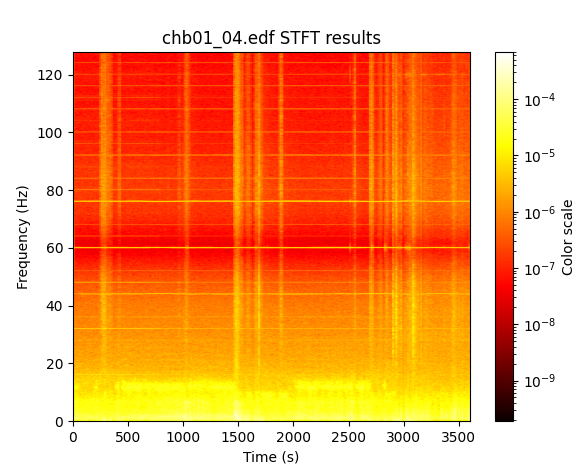
\includegraphics[width=\textwidth]{stft1}
\centering
\caption{An STFT window with high frequency resolution.}
\label{fig:stft1}
\end{figure}

\begin{figure}[H]
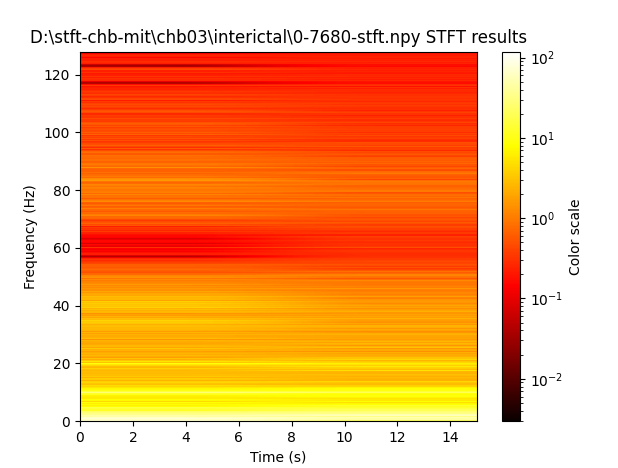
\includegraphics[width=\textwidth]{stft2}
\centering
\caption{An STFT window with high time resolution.}
\label{fig:stft2}
\end{figure}

\begin{figure}[H]
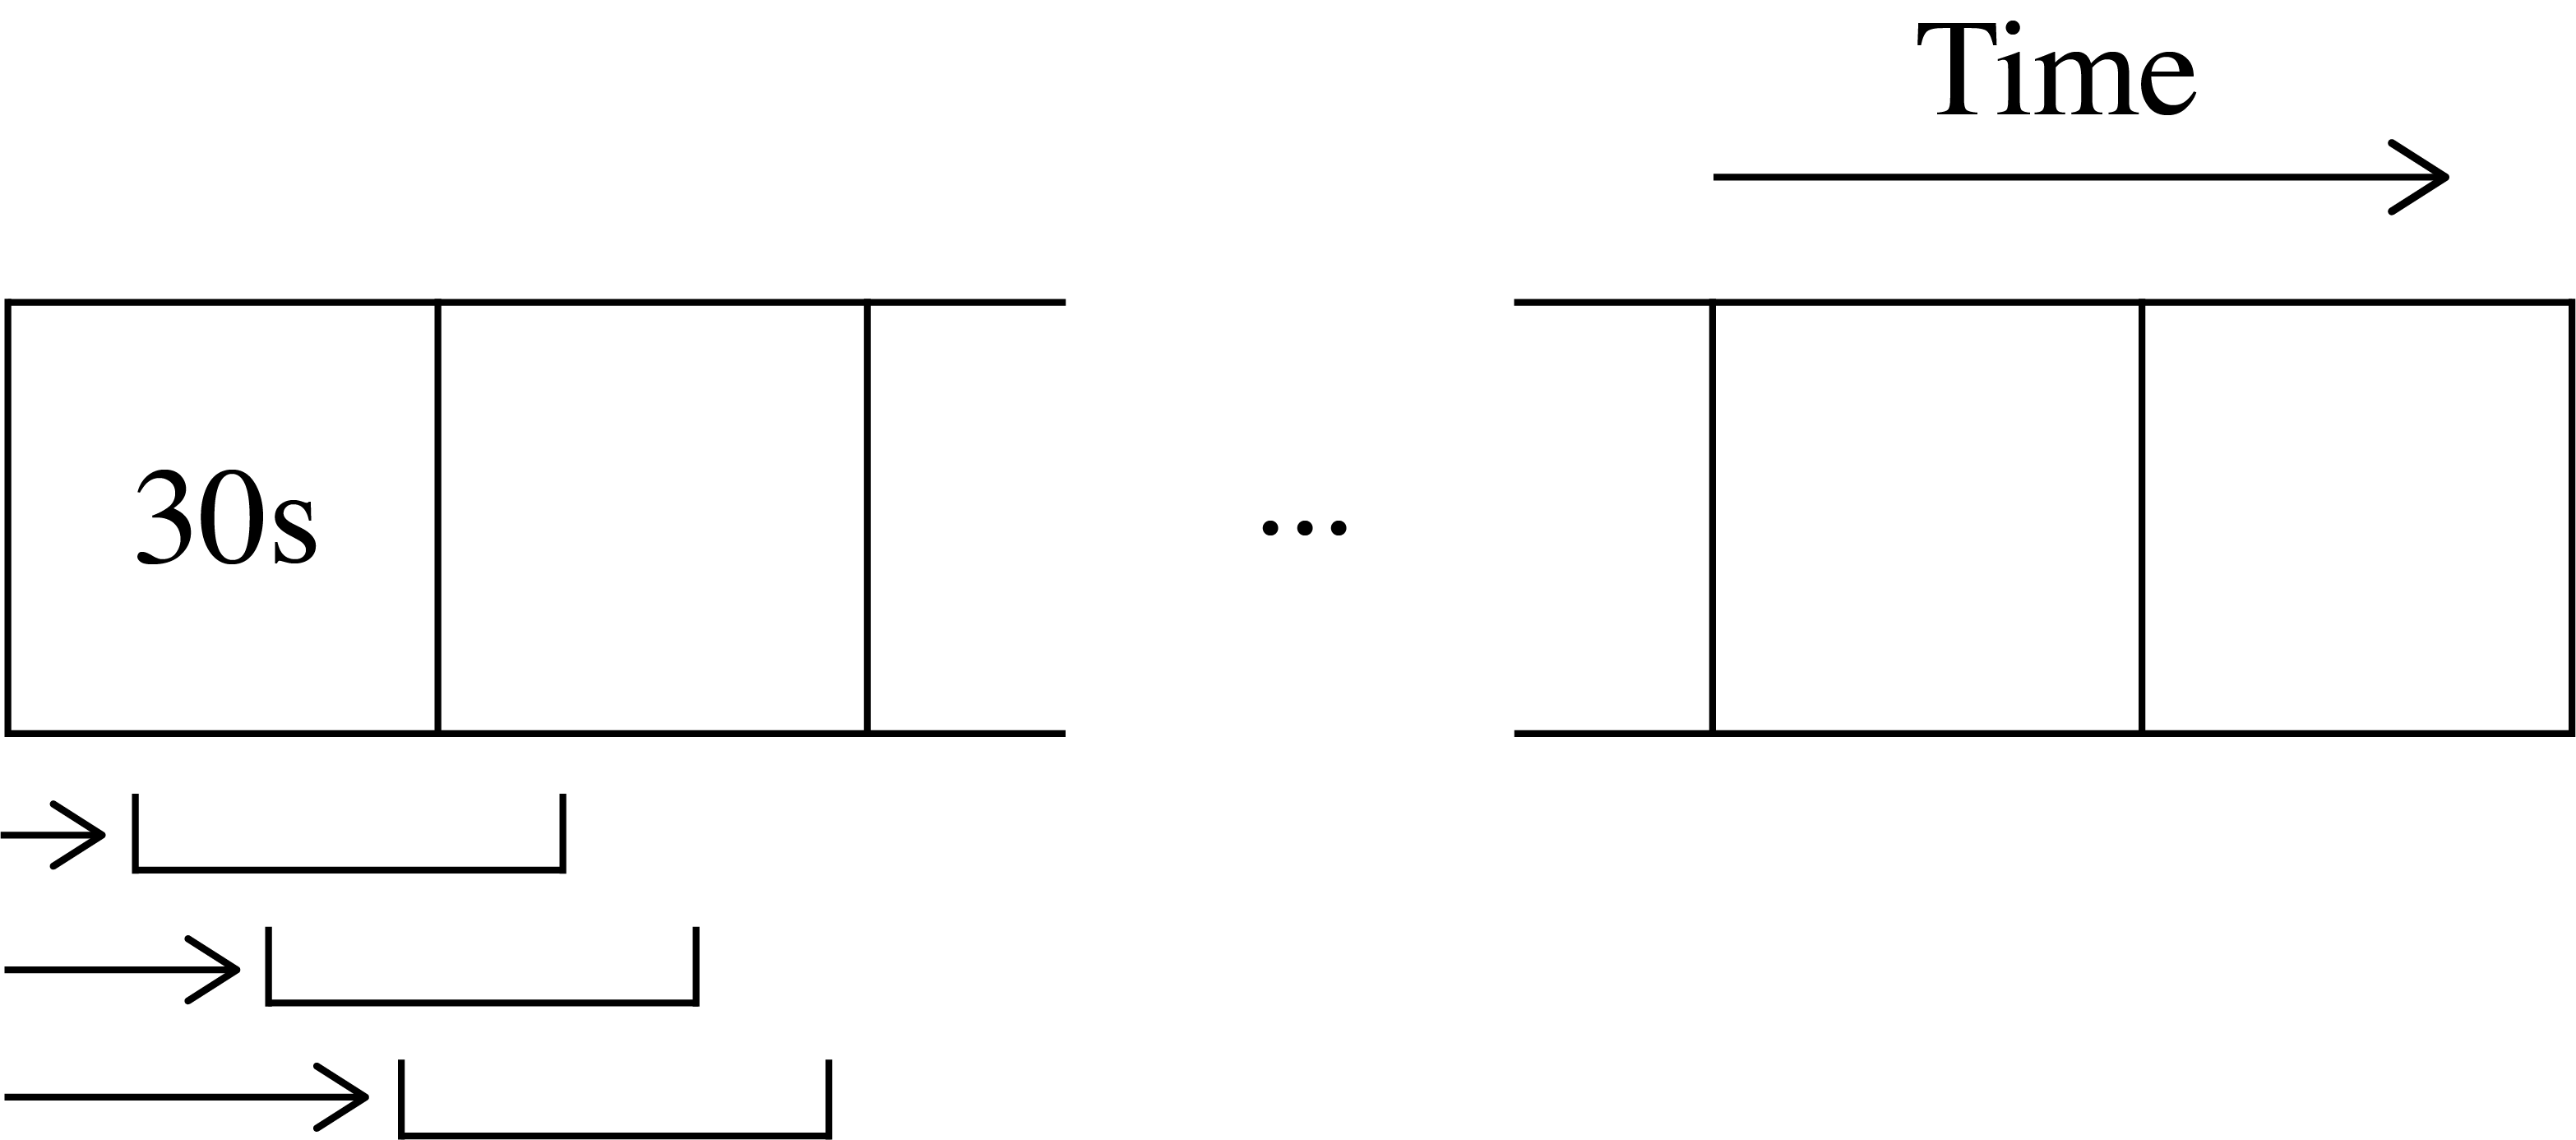
\includegraphics[width=\textwidth]{slidingWindow}
\centering
\caption{Sliding Window technique for synthesizing data spectrogram images}
\label{fig:slidingWindow}
\end{figure}

\end{document}